


%%% FOR PRESENTATION UNCOMMENT NEXT LINE
%\documentclass{beamer}
%%% FOR PRINTING SLIDE UNCOMMENT NEXT LINE 
\documentclass[handout]{beamer} 

%  **************************************************************
% Select a theme
%%%%%%%%%%%%%%%%%%%%%%%%%%%
%\usetheme{AnnArbor}
%\usetheme{Boadilla}
  \usetheme{Frankfurt}
  %\usetheme{Singapore}
%\usetheme{Madrid}
%\usetheme{Antibes}
  %\usetheme{Berkeley}
%  \usetheme{default}
  
  \usetheme{CambridgeUS}
% \usetheme{Szeged}

%%%%%%%%%%%%%%%%%%%%%%%%%%%

% Select a color theme
%%%%%%%%%%%%%%%%%%%%%%%%%%%

%  \usecolortheme{beaver}
% \usecolortheme{whale}
%  \usecolortheme{seagull}
%  \usecolortheme{dove}
%  \usecolortheme{crane} 
 % \usecolortheme{default}
  
  %\usecolortheme[rgb={.4,0,0}]{structure} % Red colors
  % \usecolortheme[rgb={.2,0,0}]{structure} % Dark Red colors
  %\usecolortheme[rgb={.6,.5,.2}]{structure} % Yellow/Green colors
  %\usecolortheme[rgb={.80,.10,.30}]{structure} % 
% \usecolortheme[rgb={.0,.0,.7}]{structure} % 

%%%%%%%%%%%%%%%%%%%%%%%%%%%
  
 % Select a font theme
 %%%%%%%%%%%%%%%%%%%%%%%%%%
   % \usefonttheme{structurebold}
    \usefonttheme{structuresmallcapsserif}
   % \usefonttheme{structureitalicserif}
   %  \usefonttheme{serif}
 %%%%%%%%%%%%%%%%%%%%%%%%%%

 % Select a background color  
 %%%%%%%%%%%%%%%%%%%%%%%%%%%%%%
   %\setbeamertemplate{background canvas}[vertical shading][bottom=white,top=gray!20]
   % \setbeamertemplate{background canvas}[vertical shading][bottom=white,top=red!10!black!30]
   
%   \setbeamertemplate{background canvas}[vertical shading][bottom=white,top=green!15!black!15]
   
    \setbeamertemplate{background canvas}[vertical shading][bottom=white,top=white]
%%%%%%%%%%%%%%%%%%%%%%%%%%%%%%%

% Select a color for math text
%%%%%%%%%%%%%%%%%%%%%%%%%%%%%%% 
 \setbeamercolor{math text}{fg=black!10!blue}
%%%%%%%%%%%%%%%%%%%%%%%%%%%%%%%

% Select a color for block
  \setbeamercolor{block title}{bg=blue!40!white, fg=black}
%  \setbeamercolor{block body}{bg=blue!5!white,fg=black}%bg=background, fg= foreground

% This command suppresses the navigation symbols at footline
% comment the command below if you  want navigation symbols 
\setbeamertemplate{navigation symbols}{}

% Set the size of the font in frame title
\setbeamerfont{frametitle}{size=\normalsize}


% This command will generate a gray footline with the ASU logo in
% each frame
  \useoutertheme{mathASUlogo}
  
%  **************************************************************
%\input{BEAMERoptions.tex}	

\usepackage{graphicx}
\usepackage{algorithmic}
\usepackage{algorithm}
\usepackage{listings}
\usepackage{verbatim}
\usepackage{moreverb}
\usepackage{movie15}
\usepackage{color, colortbl}
\usepackage{multirow}
\usepackage{slashbox}
\usepackage{stmaryrd}
\usepackage{listings}

\usepackage{tikz}
\usetikzlibrary{arrows,backgrounds}
\tikzstyle{block}=[draw opacity=0.7,line width=1.4cm]

\graphicspath{{../../CursosUGM/CursoUGM2015/Figuras/}{../../Figuras/}}

%\graphicspath{{../../Figuras/}}


\newcommand{\tensor}[1]{\underline{\underline{#1}}}
\newcommand{\Vector}[1]{\vec{#1}}
\newcommand{\mathbi}[1]{\textbf{\em #1}}
\newcommand{\mbi}[1]{\textbf{\em #1}}
\newcommand{\mbiu}[1]{_{\textbf{\em #1}}}
\newtheorem{mydef}{Definition}

\newcommand{\dt}{\partial t}
\newcommand{\dphi}{\partial \phi}
\newcommand{\ddphi}{\partial^2 \phi}
\newcommand{\dxj}{\partial x_j}
\newcommand{\dxi}{\partial x_i}
\newcommand{\dd}[1]{% arg1: some variable
	\ensuremath{ \partial #1 } }
\newcommand{\conv}[1]{% arg1: neighbors = e,w,n,s,f,b
	\ensuremath{ c_{\boldsymbol{#1}} } }
\newcommand{\diff}[2][x]{% 
\ensuremath{ \left(\frac{\partial \phi}{\partial #1}\right)_{\boldsymbol{#2}}}}
\newcommand{\vel}[2][u]{% arg1: u,v,w; arg2: neighbors = e,w,n,s,f,b
\ensuremath{ #1_{\boldsymbol{#2}} } }
\newcommand{\deltas}[2][x]{% arg1: x, y, z; arg1: neighbors = e,w,n,s,f,b
\ensuremath{ \Delta #1_{\boldsymbol{#2}} } }
\newcommand{\sphi}[1]{% arg1: neighbors = e,w,n,s,f,b,_E,_W,_N,_S,_F,_B,_P
	\ensuremath{ \phi_{\boldsymbol{#1}} } }
\newcommand{\sla}[1]{% arg1: neighbors = _E,_W,_N,_S,_F,_B,_P
	\ensuremath{ a_{\boldsymbol{#1}} } }
\newcommand{\coef}[2][a]{% arg2: neighbors = e,w,n,s,f,b,_E,_W,_N,_S,_F,_B,_P
	\ensuremath{ #1_{\boldsymbol{#2}} } }
\newcommand{\dvdt}{
	\ensuremath{ \textrm{\scriptsize{$\frac{\Delta V}{\Delta t}$}} } }
	
\newtheorem{defi}{\textit{\textbf{Definici\'on}}}[section]
\newtheorem{ejemplo}{\textit{\textbf{Ejemplo}}}[section]
\newtheorem{teorema}{\textit{\textbf{Teorema}}}[section]

% the beginning of each subsection:
\AtBeginSubsection[]
{
  \begin{frame}<beamer>{Table of contents}
    \tableofcontents[currentsection,currentsubsection]
  \end{frame}
}

%\setbeameroption{show notes}

\title[MMC II]{Modelaci\'on Matem\'atica y Computacional I \\
%\textcolor{Lured}{\footnotesize{...}}
}   
\author[LMCS]{Luis M. de la Cruz Salas \\ \textcolor{blue}{\textsf{luiggi@igeofisica.unam.mx}}} 
\institute[UNAM] 
{ 
  {\small{Grupo de Geof\'isica Matem\'atica y Computacional}} \\
  \vspace{0.15cm}
  {\small{Instituto de Geof\'isica}} \\ 
  \vspace{0.15cm}
{\small{Universidad Nacional Aut\'onoma de M\'exico}} \\
  \vspace{0.15cm}
\includegraphics[height=.85cm]{university-logo-filename.png} 
}

\date[2015]{\textcolor{Lured}{\footnotesize{Posgrado en Ciencias de la Tierra}} \\ \textcolor{Lured}{\footnotesize{
Posgrado en Ciencia e Ingenier\'{\i}a de la Computaci\'on}}}

\subtitle{\textcolor{Lured}{Soluci\'on num\'erica de ecuaciones diferenciales: MDF }}

\subject{Scientific Computing}

% \pgfdeclareimage[height=0.5cm]{university-logo}{university-logo-filename}
% \logo{\pgfuseimage{university-logo}}


% Delete this, if you do not want the 
% Pop up the table of contents at the beginning of each subsection:
\AtBeginSubsection[]
{
%  \begin{frame}<beamer>{Contenido}
  \begin{frame}
    \tableofcontents[currentsection,currentsubsection]
  \end{frame}
}


% To uncover everything in a step-wise fashion:
%\beamerdefaultoverlayspecification{<+->}


\begin{document}

\begin{frame}
  \titlepage
\end{frame}

\begin{frame}{Contenido}
  \tableofcontents
\end{frame}


\section{M\'etodo de Diferencias Finitas}

\begin{frame}
  \begin{itemize}[<+->]
  \item Diferencias Finitas (FD) es la t\'ecnica de aproximaci\'on de soluciones de EDPs
    m\'as vieja. 
    \begin{itemize}
    \item Desarrollada por Euler en 1768.
    \end{itemize}
  \item La idea es muy simple y se basa en la estimaci\'on de la derivada de una funci\'on 
    mediante la raz\'on de dos diferencias:
    \begin{itemize}
    \item Para una funci\'on $u(x)$ la derivada en el punto $x$ est\'a definida por:
      \[
      u_x \equiv \left( \frac{\partial u}{\partial x} \right) =
      \lim_{\Delta x \to 0} \frac{u(x+\Delta x) - u(x)}{\Delta x}.
      \]
    \noindent Si $\Delta x$ es peque\~na pero finita, la expresi\'on de la derecha es
    una aproximaci\'on al valor exacto $u_x$.
    $$\includegraphics[width=6cm]{malla1FD.png}$$
    \item Notaci\'on: $u(x_i) \equiv u_i$; $u(x_i+\Delta x) \equiv u(x_{i+1}) \equiv u_{i+1}$
    \item Lo mismo aplica para las derivadas: $u_x(x_i) \equiv (u_x)_i$.
    \end{itemize}
  \end{itemize}
\end{frame}

\begin{frame}
  \begin{itemize}[<+->]
  \item La aproximaci\'on en FD se mejora reduciendo $\Delta x$. 
    \begin{itemize}
    \item Para una valor finito
      de $\Delta x$ se introduce un error (truncamiento) el cual tiende a cero si 
      $\Delta x \to 0$.
    \item La potencia de $\Delta x$ con la cual el error tiende a cero es el orden de la
      aproximaci\'on.
    \end{itemize}
  \item Todo el concepto de FD est\'a basado en expansiones de Taylor: cualquier funci\'on
    continua y diferenciable, en la vecindad de $x_i$ puede ser expresada como:
{\small{
    \[
    \phi(x) = \phi(x_i) + (x-x_i)\left(\frac{\partial \phi}{\partial x}\right)_i
    + \frac{(x-x_i)^2}{2!}\left(\frac{\partial^2 \phi}{\partial x^2}\right)_i
    \]
    \[
    + \frac{(x-x_i)^3}{3!}\left(\frac{\partial^3 \phi}{\partial x^3}\right)_i + \dots
    + \frac{(x-x_i)^n}{n!}\left(\frac{\partial^n \phi}{\partial x^n}\right)_i + H
    \]
}}

\noindent donde $H$ significa el t\'ermino de m\'as alto orden.
  \end{itemize}
\end{frame}

\begin{frame}
  \begin{itemize}[<+->]
  \item Si desarrollamos $u(x+\Delta x)$ obtenemos:
    \[
    u(x+\Delta x) = u(x) + \Delta x u_x(x) + \frac{\Delta x^2}{2} u_{xx} + \dots
    \]
    \[
    \Longrightarrow
    \frac{u(x+\Delta x)-u(x)}{\Delta x} = u_x(x) + \frac{\Delta x}{2} u_{xx} + \dots
    \]

  \item El m\'as alto orden en esta aproximaci\'on es $\Delta x$, por lo que se dice
    que es de primer orden y se escribe:
    \[
    \frac{u(x+\Delta x)-u(x)}{\Delta x} = u_x(x) + \mathcal{O}(\Delta x)
    \]
  \item Esto indica que el error va a cero como la primera potencia de $\Delta x$.
  \item Se pueden obtener varias aproximaciones para las derivadas de una funci\'on de
    diferentes \'ordenes.
  \end{itemize}
\end{frame}


\begin{frame}{Backward, Forward, Central}

\begin{columns}
\begin{column}{0.52\textwidth}
\begin{footnotesize}
  \begin{itemize}[<+->]
  \item Forward (1ra derivada):
    \[
    (u_x)_i \approx \frac{u(x+\Delta x)-u(x)}{\Delta x} = \frac{u_{i+1}-u_{i}}{x_{i+1}-x_{i}} = \frac{\delta^{+} u(x)}{x_{i+1}-x_{i}} = D_+u(x)
    \]
  \item Backward (1ra derivada):
    \[
    (u_x)_i \approx \frac{u_{i}-u_{i-1}}{x_{i}-x_{i-1}} = \frac{\delta^{-} u(x)}{x_{i}-x_{i-1}} = D_-u(x)
    \]
  \item Central (1ra derivada):
    \[
    (u_x)_i \approx \frac{u_{i+1}-u_{i-1}}{x_{i+1}-x_{i-1}} = D_0u(x)
    \]
  \item Central (2da derivada):
    \[
    (u_{xx})_i \approx \frac{u_{i-1} - 2u_i + u_{i+1}}{(x_{i+1}-x_{i})(x_{i}-x_{i-1})}
     \]
  \end{itemize}
\end{footnotesize}
\end{column}
\begin{column}{0.48\textwidth}
\vspace{2cm}
$$\includegraphics[height=5.0cm, width=6.0cm]{PendientesFDM}$$
\end{column}
\end{columns}

\end{frame}


\begin{frame}
  \begin{itemize}[<+->]
  \item F\'ormulas para las derivadas se pueden obtener para cualquier n\'umero de puntos
    adyacentes.
  \item El orden de aproximaci\'on crece con el n\'umero de puntos, y de igual manera,  
    la banda del sistema diagonal es proporcional a este n\'umero de puntos.
  \item Por ejemplo:
    \[
    (u_x)_i=\frac{au_i + bu_{i-1}+cu_{i-2}}{\Delta x} + \mathcal{O}(\Delta x^2)
    \]
  \item Hay que encontrar los coeficientes $a,b$ y $c$:
{\small{
    \[
    u_{i-2}=u_i - 2\Delta x (u_x)_i + 2\Delta x^2 (u_{xx})_i - 
    \frac{(2\Delta x)^3}{6} (u_{xxx})_i + \dots 
    \]
    \[
    u_{i-1}=u_i - \Delta x (u_x)_i + \frac{\Delta x^2}{2} (u_{xx})_i - 
    \frac{\Delta x^3}{6} (u_{xxx})_i + \dots 
    \]
}}
  \end{itemize}
\end{frame}

\begin{frame}
  \begin{itemize}[<+->]
  \item Sustituyendo y haciendo un poco de \'algebra: 
    \[
    (u_x)_i=\frac{3u_i - 4u_{i-1} + u_{i-2}}{2 \Delta x} + \mathcal{O}(\Delta x^2)    
    \]
  \item Si se usan los puntos $i+2, i+1, i$ se obtiene:
    \[
    (u_x)_i=\frac{-3u_i + 4u_{i+1} - u_{i+2}}{2 \Delta x} + \mathcal{O}(\Delta x^2)    
    \]
  \end{itemize}
\end{frame}

\begin{frame}{Error de truncamiento}

Sea $u(x) = \sin(x)$. Aproximemos $u^{\prime}(x) = \cos(x)$ en $\bar{x} = 1$, es decir $\cos(1) = 0.5403023$. \uncover<2->{Los errores se dan en la siguiente tabla:}

\begin{columns}
\begin{column}{0.55\textwidth}
\uncover<2->{$$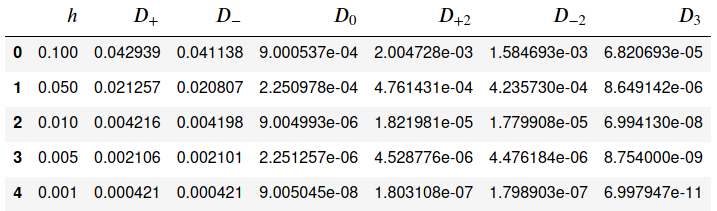
\includegraphics[scale=0.30]{TablaErroresFDM}$$}
\uncover<3->{$$\includegraphics[scale=0.30]{LogLogFDM}$$}
\end{column}
\begin{column}{0.45\textwidth}
\uncover<2->{
\begin{scriptsize}
($D_3u = \frac{1}{6h}[2u_{i+1} + 3u_i - 6u_{i-1} + u_{i-2}]$)
\[
\begin{array}{ccc}
D_+u(\bar{x}) - u^\prime(\bar{x}) & \approx & -0.42 h \\
D_0u(\bar{x}) - u^\prime(\bar{x}) & \approx & -0.09 h^2 \\
D_3u(\bar{x}) - u^\prime(\bar{x}) & \approx & -0.007 h^3 
\end{array}
\]
\end{scriptsize}
}
\uncover<4->{
\begin{small}
Si el error se comporta como $E(h) \approx C h^p$ entonces

\[
\log(E(h)) \approx \log|C| + p \log h 
\]

La pendiente de la l\'inea recta es $p$, es decir, el orden de la aproximaci\'on.

N\'otese que $\Delta x \equiv h$.
\end{small}

\vspace{1cm}

}
\end{column}
\end{columns}

\end{frame}

\subsection{Problemas estacionarios}

\begin{frame}{Ecuaci\'on de Poisson 1D}

\textsf{N} $\equiv$ N\'umero de inc\'ognitas. \textsf{N+1} $\equiv$ N\'umero de celdas. 

$$\includegraphics[width=10cm]{malla1D_DF.png}$$

\pause

\begin{columns}
\begin{column}{0.45\textwidth}
\[
\frac{\partial^2 u}{\partial x^2} = f
\]
Condiciones de frontera tipo Dirichlet: 
\begin{eqnarray*}
u_0 & = & A\\ 
u_{N+1} & = & B
\end{eqnarray*}
Llamaremos a $\hat{u}(x)$ la soluci\'on exacta del problema.
\end{column}
\begin{column}{0.45\textwidth}

\pause 

Aprox. en Diferencias Finitas
\[
  (u_{xx})_i \approx \frac{u_{i+1} - 2 u_{i} + u_{i-1}}{\Delta x^2}
\]
Donde $\Delta x = L / (\textsf{N+1}) \equiv h$

\[
\boxed{u_{i-1} - 2 u_{i} + u_{i+1} = h^2 f_i}
\]

\end{column}
\end{columns}

\end{frame}

\begin{frame}{Ecuaci\'on de Poisson 1D : Condiciones de frontera Dirichlet}

$$\includegraphics[width=10cm]{malla1D_DF.png}$$

\begin{small}

\begin{columns}
\begin{column}{0.45\textwidth}
$ u_0  = A $.

$u_{0} - 2 u_{1} + u_{2} = h^2 f_1$ 

$\Rightarrow \boxed{-2 u_{1} + u_{2} = h^2 f_1 - A}$
\end{column}
\begin{column}{0.45\textwidth}
$ u_{N+1}  = B$

$u_{N-1} - 2 u_{N} + u_{N+1} = h^2 f_N$

$\Rightarrow \boxed{u_{N-1} - 2 u_{N} = h^2 f_N - B}$
\end{column}
\end{columns}

\pause

\strut
\[ 
\Longrightarrow
\underbrace{
\left[
  \begin{matrix}
    -2 & 1 & 0 & 0 & \dots & 0  \\
    1 & -2 & 1 & 0 & \dots & 0  \\
    0 & 1 & -2 & 1 & \dots & 0  \\
    \vdots & \ddots & \ddots & \ddots & \ddots & \vdots \\
    0 & \dots & 0 & 1 & -2 & 1   \\
    0 & \dots & 0 & 0 & 1 & -2    
  \end{matrix}
\right]}_{N \times N}
\left[
\begin{matrix}
u_1 \\ u_2 \\ u_3 \\ \vdots \\ u_{N-1} \\ u_N
\end{matrix}
\right]= 
h^2 \left[
\begin{matrix}
f_1 \\ f_2 \\ f_3 \\ \vdots \\ f_{N-1} \\ f_N
\end{matrix}
\right] +
\left[
\begin{matrix}
-A \\ 0 \\ 0 \\ \vdots \\ 0 \\ -B
\end{matrix}
\right]
\]
\end{small}

\end{frame}


\lstset{language=python}
\lstset{keywordstyle=\color{blue}}
%\lstset{backgroundcolor=\color{darkgray}}
\lstset{basicstyle=\tiny}
%\lstset{emph={File,interactive,UnitSquare,Expression,FacetNormal,VariationalProblem,ds,grad,inner,dx,vector,solve,assemble,apply,assign,plot,TestFunction,TrialFunction,Function,Rectangle,FunctionSpace,Constant,DirichletBC,interpolate},emphstyle=\color{red}}
\lstset{commentstyle=\textit}
\lstset{frame=trbl}

\begin{frame}[fragile]{Python: Construcci\'on del sistema (\texttt{Poisson1D\_01.py})}

\begin{columns}
	\begin{column}{0.5\textwidth}
{\footnotesize \[
\underbrace{\left[
\begin{matrix}
	-2 & 1 & 0 & 0 & \dots & 0  \\
	1 & -2 & 1 & 0 & \dots & 0  \\
	0 & 1 & -2 & 1 & \dots & 0  \\
	\vdots & \ddots & \ddots & \ddots & \ddots & \vdots \\
	0 & \dots & 0 & 1 & -2 & 1   \\
	0 & \dots & 0 & 0 & 1 & -2    
\end{matrix}
\right]}_{N \times N}
\]}
	\end{column}
	\begin{column}{0.5\textwidth}  %%<--- here

\begin{lstlisting}
import numpy as np

def Laplaciano1D(N, diagonal):
    A = np.zeros((N,N))
    A[0,0] = diagonal; A[0,1] = 1
    for i in range(1,N-1):
        A[i,i] = diagonal
        A[i,i+1] = 1
        A[i,i-1] = 1
    A[N-1,N-2] = 1; A[N-1,N-1] = diagonal
return A

A = Laplaciano1D(N, -2)
\end{lstlisting}		

	\end{column}
\end{columns}

\pause

\begin{columns}
	\begin{column}{0.5\textwidth}
{\footnotesize 		\[
		h^2 \underbrace{\left[
		\begin{matrix}
		0 \\ 0 \\ 0 \\ \vdots \\ 0 \\ 0
		\end{matrix}
		\right]}_f +
		\left[
		\begin{matrix}
		-A \\ 0 \\ 0 \\ \vdots \\ 0 \\ -B
		\end{matrix}
		\right]
		\]}
	\end{column}
	\begin{column}{0.5\textwidth}  %%<--- here		
\[
f = 0, \,\, u_0 = A, \,\, u_{N+1} = B
\]		

\begin{lstlisting}
f = np.zeros(N)
f[0] -= boundA   # f[0] = f[0] - boundA 
f[N-1] -= boundB # f[N-1] = f[N-1] - boundB	
\end{lstlisting}

	\end{column}
\end{columns}

\end{frame}

\begin{frame}[fragile]{Python: Soluci\'on del sistema y graficaci\'on}
	
	\begin{columns}
		\begin{column}{0.3\textwidth}
			{\footnotesize \[
			\left[
			\begin{matrix}
			u_1 \\ u_2 \\ u_3 \\ \vdots \\ u_{N-1} \\ u_N
			\end{matrix}
			\right]\]}
		\end{column}
		\begin{column}{0.7\textwidth}  %%<--- here
			
\begin{lstlisting}
u[1:N+1] = np.linalg.solve(A,f)
u[0] = boundA
u[N+1] = boundB 
\end{lstlisting}	
{\tiny
\[
\begin{array}{|r|ccccc|}
\hline
\texttt{x} \rightarrow & x_0 & x_1 & \dots & x_N & x_{N+1}  \\
\hline 
\texttt{u} \rightarrow & u_0 & u_1 & \dots & u_N & u_{N+1}  \\
\hline 
\texttt{f} \rightarrow &     & f_0 & \dots & f_{N-1} &     \\
\hline 
\texttt{A[0]} \rightarrow &  & A_{0,0} & \dots &  A_{0,N-1} & \\
 & & \vdots & \ddots & \vdots &  \\
\texttt{A[N-1]} \rightarrow & & A_{N-1,0} & \dots &  A_{N-1,N-1} &\\
\hline
\end{array}
\]
}		
		\end{column}
	\end{columns}
	
\pause

	\begin{columns}
		\begin{column}{0.5\textwidth}
$$\includegraphics[width=5cm]{solucion01.png}$$
		\end{column}
		\begin{column}{0.5\textwidth}  %%<--- here			
			
\begin{lstlisting}
import matplotlib.pyplot as plt

x = np.linspace(a,b,N+2)
plt.plot(x,u,'-bo')
plt.show()
\end{lstlisting}

{\footnotesize 
$a = 0, \,\, b = 1, \,\, N = 20$ ($h = 0.047619$)

$A = 2.0, \,\, B = 1.0$}
		\end{column}
	\end{columns}
	
\end{frame}

\begin{frame}{Poisson 1D con $\Gamma \neq constante$}
	
{\small 

\begin{columns}
	
\begin{column}{0.5\textwidth}
	\begin{displaymath}
	\dfrac{d}{d x} \left(\Gamma \dfrac{d u}{d x} \right) = 0, \,\,\, \Gamma = |sin(4 \pi x)|
	\end{displaymath}
\end{column}
\begin{column}{0.5\textwidth}
	$$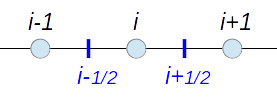
\includegraphics[width=4cm]{malla1D_DF_Centrales.png}$$
\end{column}

\end{columns}

\pause

\begin{displaymath}
g = \Gamma \dfrac{d u}{d x} \Longrightarrow \dfrac{d}{d x} \left(\Gamma \dfrac{d u}{d x} \right) = \dfrac{d g}{d x} 
\Longrightarrow
\dfrac{d g}{d x} \Big|_{i} = \dfrac{g_{i+\frac{1}{2}} - g_{i-\frac{1}{2}}}{h} =
\dfrac{\left[\Gamma \frac{du}{dx}\right]_{i+\frac{1}{2}} - \left[\Gamma \frac{du}{dx}\right]_{i-\frac{1}{2}}}{h}
\end{displaymath}

\pause

\begin{displaymath}
\left[\Gamma \frac{du}{dx}\right]_{i+\frac{1}{2}} = 
\Gamma_{i+\frac{1}{2}} \left[\dfrac{u_{i+1}-u_{i}}{h}\right] =
\dfrac{1}{h}\left[\Gamma_{i+\frac{1}{2}} u_{i+1} - \Gamma_{i+\frac{1}{2}} u_{i}\right]
\end{displaymath}

\begin{displaymath}
\left[\Gamma \frac{du}{dx}\right]_{i-\frac{1}{2}} = 
\Gamma_{i-\frac{1}{2}} \left[\dfrac{u_{i}-u_{i-1}}{h}\right] =
\dfrac{1}{h}\left[\Gamma_{i-\frac{1}{2}} u_{i} - \Gamma_{i-\frac{1}{2}} u_{i-1}\right]
\end{displaymath}
}

\end{frame}

\begin{frame}{Poisson 1D con $\Gamma \neq constante$}
	
{\small 

$$\includegraphics[width=10cm]{malla1D_DF.png}$$

\begin{displaymath}
\dfrac{1}{h^2} \left[
\Gamma_{i+\frac{1}{2}} u_{i+1} - 
(\Gamma_{i+\frac{1}{2}} + \Gamma_{i-\frac{1}{2}}) u_{i} +
\Gamma_{i-\frac{1}{2}} u_{i-1}
\right] = 0
\end{displaymath}

\pause

donde 

\begin{displaymath}
\Gamma_{i+\frac{1}{2}} = \dfrac{ \Gamma_{i+1} + \Gamma_{i}}{2} \,\,\, \text{ y } \,\,\,
\Gamma_{i-\frac{1}{2}} = \dfrac{ \Gamma_{i-1} + \Gamma_{i}}{2}
\end{displaymath}

\pause

\begin{displaymath}
i = 1 \,\,\, \Longrightarrow \,\,\,
\Gamma_{1+\frac{1}{2}} u_{2} - 
(\Gamma_{1+\frac{1}{2}} + \Gamma_{1-\frac{1}{2}}) u_{1} = - 
\Gamma_{1-\frac{1}{2}} u_{0}
\end{displaymath}

\begin{displaymath}
i = N \,\,\, \Longrightarrow \,\,\,
- (\Gamma_{N+\frac{1}{2}} + \Gamma_{N-\frac{1}{2}}) u_{N} +
\Gamma_{N-\frac{1}{2}} u_{N-1} = 
- \Gamma_{N+\frac{1}{2}} u_{N+1}
\end{displaymath}

}

\end{frame}


\begin{frame}[fragile]{Python: $\Gamma \neq constante$ (\texttt{Poisson1D\_01\_Gamma.py})}

\begin{lstlisting}
def Laplaciano1D(N, diagonal):
    A = np.zeros((N,N))
    A[0,0] -= (0.5 * diagonal[0] + diagonal[1] + 0.5 * diagonal[2])
    A[0,1] = 0.5 * (diagonal[1] + diagonal[2])
    for i in range(1,N-1):
        A[i,i] -= (0.5 * diagonal[i+2] + diagonal[i+1] + 0.5 * diagonal[i])
        A[i,i+1] = 0.5 * (diagonal[i+1] + diagonal[i+2])
        A[i,i-1] = 0.5 * (diagonal[i+1] + diagonal[i])
    A[N-1,N-2] = 0.5 * (diagonal[N-1] + diagonal[N]) 
    A[N-1,N-1] -= (0.5 * diagonal[N-1] + diagonal[N] + 0.5 * diagonal[N+1]);
return A

gamma = np.abs(np.sin(4 * np.pi * x))
A = Laplaciano1D(N, gamma)

f = np.zeros(N)       
f[0] -= boundA * (gamma[0] + gamma[1]) * 0.5
f[N-1] -= boundB * (gamma[N] + gamma[N+1]) * 0.5
\end{lstlisting}

{\tiny
\[
\begin{array}{|r|cccccccc|}
\hline
\texttt{x} \rightarrow & x_0 & x_1 & x_2 & x_3 & \dots & x_{N-1} & x_N & x_{N+1}  \\
\hline 
\texttt{u} \rightarrow & u_0 & u_1 & u_2 & u_3 & \dots & u_{N-1} & u_N & u_{N+1}  \\
\hline
\Gamma \rightarrow & \Gamma_0 & \Gamma_1 & \Gamma_2 & \Gamma_3 & \dots & \Gamma_{N-1} & \Gamma_N & \Gamma_{N+1}  \\
\hline 
\texttt{f} \rightarrow &  & f_0 & f_1 & f_2 & \dots & f_{N-2} & f_{N-1} &     \\
\hline 
\texttt{A[0]} \rightarrow & & A_{0,0} & A_{0,1} & A_{0,2} & \dots & A_{0,N-2} &  A_{0,N-1} &\\
%\texttt{A[1]} \rightarrow & & A_{1,0} & A_{1,1} & A_{1,2} & \dots & A_{1,N-2} &  A_{1,N-1} &\\
    & & \vdots & \vdots & \vdots & \ddots & \vdots & \vdots & \\
\texttt{A[N-1]} \rightarrow & & A_{N-1,0} & A_{N-1,1} & A_{N-1,2} & \dots & A_{N-1,N-2} &  A_{N-1,N-1} &\\
\hline
\end{array}
\]
}

\end{frame}

\begin{frame}[fragile]{Python: $\Gamma \neq constante$}

{\footnotesize 
$a = 0, \,\, b = 1, \,\, N = 50 (h = 0.0196078), \,\, A = 2.0, \,\, B = 1.0, \,\, \Gamma = |sin(4 \pi x)|$
}
	\begin{columns}
		\begin{column}{0.5\textwidth}
			$$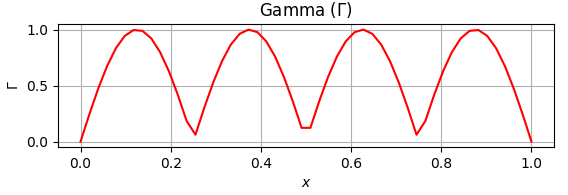
\includegraphics[width=6cm]{gamma.png}$$
		\end{column}
		\begin{column}{0.5\textwidth}  %%<--- here			
			$$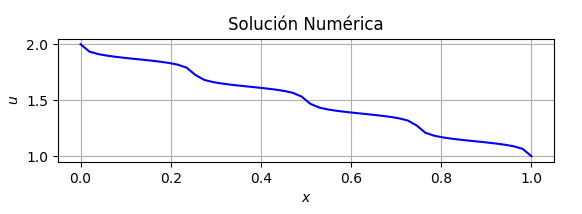
\includegraphics[width=6cm]{solucion02.png}$$
		\end{column}
	\end{columns}

{\footnotesize 
	$a = 0, \,\, b = 1, \,\, N = 50 (h = 0.0196078), \,\, A = 2.0, \,\, B = 1.0, \,\, \Gamma = \texttt{random(x)}$
}
	\begin{columns}
		\begin{column}{0.5\textwidth}
			$$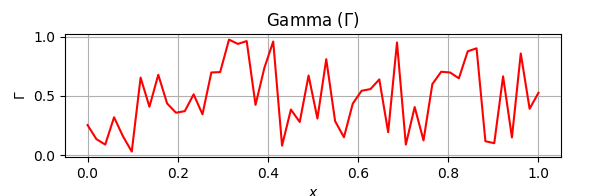
\includegraphics[width=6cm]{gamma3.png}$$
		\end{column}
		\begin{column}{0.5\textwidth}  %%<--- here			
			$$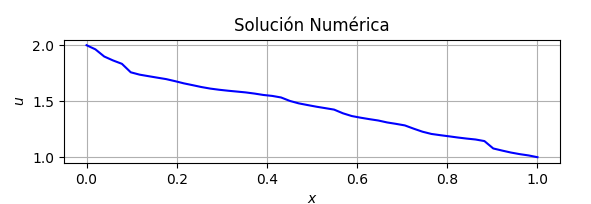
\includegraphics[width=6cm]{solucion03.png}$$
		\end{column}
	\end{columns}
	
\end{frame}

		
\begin{frame}{Ecuaci\'on de Poisson 1D : Condici\'on de frontera Neumman I}

$$\includegraphics[width=10cm]{malla1D_DF.png}$$

\begin{footnotesize}
\begin{columns}
\begin{column}{0.45\textwidth}
$ u_0  = A $.

$u_{0} - 2 u_{1} + u_{2} = h^2 f_1$ 

$\Rightarrow \boxed{-2 u_{1} + u_{2} = h^2 f_1 - A}$
\end{column}
\begin{column}{0.5\textwidth}
$\left.\displaystyle \frac{\partial u}{\partial n}\right|_{N+1}  = B \Longrightarrow \boxed{u_{N+1} - u_{N} = h B}$  

\end{column}
\end{columns}

\pause

\strut

\[
\Longrightarrow
\underbrace{
\left[
  \begin{matrix}
    -2 & 1 & 0  & \dots & 0 & 0  \\
    1 & -2 & 1  & \dots & 0 & 0 \\
    \vdots & \ddots & \ddots & \ddots & \vdots & \vdots \\
    0 & \dots & 1 & -2 & 1 & 0 \\
    0 & \dots & 0 & 1 & -2 & 1 \\
    0 & \dots & 0 & 0 & -1 & 1        
  \end{matrix}
\right] 
}_{N+1 \times N+1}
\left[
\begin{matrix}
u_1 \\ u_2 \\ \vdots \\ u_{N-1} \\ u_N \\ u_{N+1}
\end{matrix}
\right]= 
h^2 \left[
\begin{matrix}
f_1 \\ f_2 \\ \vdots \\ f_{N-1} \\ f_N \\ 0
\end{matrix}
\right] +
\left[
\begin{matrix}
-A \\ 0 \\  \vdots \\ 0 \\ 0 \\ hB
\end{matrix}
\right]
\]

(\texttt{Poisson1D\_05.py, INPUT\_02})
\end{footnotesize}

\end{frame}

\begin{frame}{Ecuaci\'on de Poisson 1D : Condici\'on de frontera Neumman II}

$$\includegraphics[width=10cm]{malla1D_DF.png}$$

\begin{footnotesize}
\begin{columns}
\begin{column}{0.45\textwidth}
$ u_0  = A $.

$u_{0} - 2 u_{1} + u_{2} = h^2 f_1$ 

$\Rightarrow \boxed{-2 u_{1} + u_{2} = h^2 f_1 - A}$
\end{column}
\begin{column}{0.5\textwidth}
$\left.\displaystyle \frac{\partial u}{\partial n}\right|_{N+1}  = B \Longrightarrow \boxed{u_{N+1} = h B + u_{N}}$  

$u_{N-1} - 2 u_{N} + u_{N+1} = h^2 f_N$

$\Rightarrow \boxed{u_{N-1} - u_{N} = h^2 f_N - hB}$
\end{column}
\end{columns}

\pause

\vspace{0.25cm}

\[
\Longrightarrow
\underbrace{
\left[
  \begin{matrix}
    -2 & 1 & 0 & 0 & \dots & 0  \\
    1 & -2 & 1 & 0 & \dots & 0  \\
    0 & 1 & -2 & 1 & \dots & 0  \\
    \vdots & \ddots & \ddots & \ddots & \ddots & \vdots \\
    0 & 0 & 0 & 1 & -2 & 1   \\
    0 & 0 & 0 & 0 & 1 & -1    
  \end{matrix}
\right] }_{N \times N}
\left[
\begin{matrix}
u_1 \\ u_2 \\ u_3 \\ \vdots \\ u_{N-1} \\ u_N
\end{matrix}
\right]= 
h^2 \left[
\begin{matrix}
f_1 \\ f_2 \\ f_3 \\ \vdots \\ f_{N-1} \\ f_N
\end{matrix}
\right] +
\left[
\begin{matrix}
-A \\ 0 \\ 0 \\ \vdots \\ 0 \\ -hB
\end{matrix}
\right]
\]

(\texttt{Poisson1D\_02.py}), (\texttt{Poisson1D\_04.py, INPUT\_02})

\end{footnotesize}

\end{frame}

\begin{frame}{Ecuaci\'on de Poisson 1D : Condici\'on de frontera Neumman III}

$$\includegraphics[width=10cm]{malla1D_DF.png}$$

\begin{footnotesize}
\begin{columns}
\begin{column}{0.40\textwidth}
$ u_0  = A $.

$u_{0} - 2 u_{1} + u_{2} = h^2 f_1$ 

$\Rightarrow \boxed{-2 u_{1} + u_{2} = h^2 f_1 - A}$
\end{column}
\begin{column}{0.6\textwidth}
$\left.\displaystyle \frac{\partial u}{\partial n}\right|_{N+1}  = 
\boxed{\frac{1}{h}\left( \frac{3}{2} u_{N+1} - 2 u_{N} + \frac{1}{2} u_{N-1} \right) = B}$

\end{column}
\end{columns}

\pause

\vspace{0.25cm}

\[
\Longrightarrow
\underbrace{
\left[
  \begin{matrix}
    -2 & 1 & 0  & \dots & 0 & 0  \\
    1 & -2 & 1  & \dots & 0 & 0 \\
    \vdots & \ddots & \ddots & \ddots & \vdots & \vdots \\
    0 & \dots & 1 & -2 & 1 & 0 \\
    0 & \dots & 0 & 1 & -2 & 1 \\
    0 & \dots & 0 & \frac{1}{2} & -2 & \frac{3}{2}        
  \end{matrix}
\right] 
}_{N+1 \times N+1}
\left[
\begin{matrix}
u_1 \\ u_2 \\ \vdots \\ u_{N-1} \\ u_N \\ u_{N+1}
\end{matrix}
\right]= 
h^2 \left[
\begin{matrix}
f_1 \\ f_2 \\ \vdots \\ f_{N-1} \\ f_N \\ 0
\end{matrix}
\right] +
\left[
\begin{matrix}
-A \\ 0 \\  \vdots \\ 0 \\ 0 \\ hB
\end{matrix}
\right]
\]


\end{footnotesize}

\end{frame}

\begin{frame}{Ecuaci\'on de Poisson 1D : Condici\'on de frontera Neumman IV}

$$\includegraphics[width=10cm]{malla1D_DF.png}$$
\begin{footnotesize}
\begin{columns}
\begin{column}{0.40\textwidth}
$ u_0  = A $.

$u_{0} - 2 u_{1} + u_{2} = h^2 f_1$ 

$\Rightarrow \boxed{-2 u_{1} + u_{2} = h^2 f_1 - A}$
\end{column}
\begin{column}{0.6\textwidth}
$u_{N} - 2u_{N+1} + u_{N+2} = h^2 f_{N+1}$

$\left.\displaystyle \frac{\partial u}{\partial n}\right|_{N+1}  = 
\frac{1}{2h}\left( u_{N+2} - u_{N} \right) = B$

$\Longrightarrow \boxed{u_{N} - u_{N+1} = \frac{h^2}{2} f_{N+1} - hB}$
\end{column}
\end{columns}

\pause

%\vspace{0.25cm}

\[
\Longrightarrow
\underbrace{
\left[
  \begin{matrix}
    -2 & 1 & 0  & \dots & 0 & 0  \\
    1 & -2 & 1  & \dots & 0 & 0 \\
    \vdots & \ddots & \ddots & \ddots & \vdots & \vdots \\
    0 & \dots & 1 & -2 & 1 & 0 \\
    0 & \dots & 0 & 1 & -2 & 1 \\
    0 & \dots & 0 & 0 & 1 & -1        
  \end{matrix}
\right] 
}_{N+1 \times N+1}
\left[
\begin{matrix}
u_1 \\ u_2 \\ \vdots \\ u_{N-1} \\ u_N \\ u_{N+1}
\end{matrix}
\right]= 
h^2 \left[
\begin{matrix}
f_1 \\ f_2 \\ \vdots \\ f_{N-1} \\ f_N \\ f_{N+1}/2
\end{matrix}
\right] +
\left[
\begin{matrix}
-A \\ 0 \\  \vdots \\ 0 \\ 0 \\ -hB
\end{matrix}
\right]
\]

(\texttt{Poisson1D\_06.py, INPUT\_02})
\end{footnotesize}

\end{frame}

\begin{frame}{Medici\'on del error}

\begin{itemize}[<+->]
\item Dado que $\hat{u}(x)$ representa la soluci\'on exacta del problema, definimos el error en el punto $x_i$ de la aproximaci\'on como $E_i = u(x_i) - \hat{u}(x_i)$. 

\item El vector $\Vector{E} = (E_0, E_1, \dots, E_{N+1})$ representa el error en todos los puntos de la malla. La magnitud de este vector debe darnos el error global de la aproximaci\'on. 

\item Se puede usar cualquier norma para medir la magnitud, por ejemplo:

\begin{small}
\begin{itemize}
\item Norma infinito
\[
|| E ||_\infty = \max\limits_{1 \leq i \leq N}|E_i| = \max\limits_{1 \leq i \leq N} |u(x_i) - \hat{u}(x_i) |
\]

\item Norma uno
\[
||E||_1 = h \sum\limits_{i=1}^{N} |E_i|
\]

\item Norma Euclideana
\[
||E||_2 = \left(h \sum\limits_{i=1}^{N} |E_i|^2 \right)^{1/2}
\]
\end{itemize}

\end{small}

\end{itemize}

\end{frame}

\begin{frame}{Ejemplo 1: Poisson en 1D con condiciones Dirichlet}

{\small 
$$\includegraphics[width=10cm]{malla1D_DF.png}$$

\begin{eqnarray*}
\frac{d^2 u(x)}{d x^2} & = & -f^2 u(x) \,\,\,\,\, x \in [0,1] \\
u(0) & = & 1 \\
u(1) & = & 1
\end{eqnarray*}

Soluci\'on anal\'itica

\[
u(x) = \frac{1-\cos(f)}{\sin(f)} \sin(f x) + b\cos(f x)
\]

(\texttt{Poisson1D\_03.py, INPUT\_01})
}
\end{frame}


\begin{frame}{Ejemplo 2: Poisson en 1D con una condici\'on Neumman}
	
{\small 	
$$\includegraphics[width=10cm]{malla1D_DF.png}$$
	
	\begin{eqnarray*}
		\frac{d^2 u(x)}{d x^2} & = & e^x \,\,\,\,\, x \in [0,1] \\
	     \frac{du}{d n}(0) & = & 0 \\
		u(1) & = & 3
	\end{eqnarray*}
	
	Soluci\'on anal\'itica
	
	\[
	u(x) = e^x - x - e + 4
	\]

(\texttt{Poisson1D\_04.py, Poisson1D\_05.py, Poisson1D\_06.py, INPUT\_02})	
}
\end{frame}


\begin{frame}{Ecuaci\'on de Poisson 2D}

\begin{columns}
\begin{column}{0.60\textwidth}
\[
\frac{\partial^2 u}{\partial x^2} + \frac{\partial^2 u}{\partial y^2} = f
\]

\pause

\begin{eqnarray*}
(u_{xx})_{i,j} \approx \frac{u_{i+1,j} - 2 u_{i,j} + u_{i-1,j}}{\Delta x^2}; \\
(u_{yy})_{i,j} \approx \frac{u_{i,j+1} - 2 u_{i,j} + u_{i,j-1}}{\Delta y^2}.
\end{eqnarray*}
\begin{small}
Donde $\Delta x = L_x / (\textsf{N}_x + \textsf{1})$ y $\Delta y = L_y / (\textsf{N}_y + \textsf{1})$. 
\end{small}\end{column}
\begin{column}{0.40\textwidth}
$$\includegraphics[scale=0.28]{malla2D_FDM}$$
\end{column}
\end{columns}

\pause

Cuando $\Delta x = \Delta y = h$ entonces:
  \[
  \boxed{-4u_{i,j} +  u_{i+1,j} + u_{i-1,j} + u_{i,j+1} + u_{i,j-1} = h^2 f_{i,j}}
  \]
  \begin{tikzpicture}
      \draw[help lines,white] (0,0) grid (12,7);
  \end{tikzpicture}
\end{frame}

\begin{frame}{Matriz 2D : Pentadiagonales}
 
\[
\left[
\begin{array}{cccc|cccc|ccc}
-4 & 1 & 0 & 0 &  1 & 0 & 0 & 0 & 0 & 0 & \dots\\
 1 &-4 & 1 & 0 &  0 & 1 & 0 & 0 & 0 & 0 & \dots\\
 0 & 1 &-4 & 1 &  0 & 0 & 1 & 0 & 0 & 0 & \dots\\
 0 & 0 & 1 &-4 &  0 & 0 & 0 & 1 & 0 & 0 & \dots\\
 \hline
 1 & 0 & 0 & 0 & -4 & 1 & 0 & 0 & 1 & 0 & \dots\\
 0 & 1 & 0 & 0 &  1 &-4 & 1 & 0 & 0 & 1 & \dots\\
 0 & 0 & 1 & 0 &  0 & 1 &-4 & 1 & 0 & 0 & \dots\\
 0 & 0 & 0 & 1 &  0 & 0 & 1 &-4 & 0 & 0 & \dots\\
 \hline
 0 & 0 & 0 & 0 &  1 & 0 & 0 & 0 &-4 & 1 & \dots\\
 0 & 0 & 0 & 0 &  0 & 1 & 0 & 0 & 1 &-4 & \dots\\
 0 & 0 & 0 & 0 &  0 & 0 & 1 & 0 & 0 & 1 & \dots\\
 \vdots & \vdots & \vdots & \vdots & \vdots & \vdots & \vdots & \vdots & \vdots & \vdots & \ddots 
\end{array} \right]
\]

\end{frame}

\begin{frame}{Ecuaci\'on de Poisson 3D}

\begin{columns}
\begin{column}{0.70\textwidth}
\begin{small}
\[
\frac{\partial^2 u}{\partial x^2} + \frac{\partial^2 u}{\partial y^2} + \frac{\partial^2 u}{\partial z^2}= f
\]

\pause

\begin{eqnarray*}
(u_{xx})_{i,j,k} & \approx & \frac{u_{i+1,j,k} - 2 u_{i,j,k} + u_{i-1,j,k}}{\Delta x^2} ; \\
(u_{yy})_{i,j,k} & \approx & \frac{u_{i,j+1,k} - 2 u_{i,j,k} + u_{i,j-1,k}}{\Delta y^2} ; \\
(u_{zz})_{i,j,k} & \approx & \frac{u_{i,j,k+1} - 2 u_{i,j,k} + u_{i,j,k-1}}{\Delta z^2} .
\end{eqnarray*} 
Donde $\Delta x = L_x / (\textsf{N}_x + \textsf{1})$, $\Delta y = L_y / (\textsf{N}_y + \textsf{1})$
y $\Delta z = L_z / (\textsf{N}_z + \textsf{1})$. 
\end{small} 
\end{column}
\begin{column}{0.30\textwidth}
$$\includegraphics[scale=0.12]{malla3D_FDM}$$
$$\includegraphics[scale=0.20]{stencil3D_FDM}$$
\end{column}
\end{columns}

\pause

\begin{small}
Cuando $\Delta x = \Delta y = \Delta z = h$ entonces:
\[
\boxed{-6u_{i,j,k} +  u_{i+1,j,k} + u_{i-1,j,k} + u_{i,j+1,k} + u_{i,j-1,k} + u_{i,j,k+1} + u_{i,j,k-1} = h^2 f_{i,j,k}}
\]
\end{small}
  \begin{tikzpicture}
      \draw[help lines,white] (0,0) grid (12,7);
  \end{tikzpicture}
\end{frame}

\begin{frame}{Matriz 3D : Heptadiagonales}

\begin{scriptsize}
\[
\left[
\begin{array}{ccc|ccc|ccc||ccc|ccc|cc}
-6 & 1 & 0 & 1 & 0 & 0 & 0 & 0 & 0 & 1 & 0 & 0 & 0 & 0 & 0 & 0 & \dots\\
 1 &-6 & 1 & 0 & 1 & 0 & 0 & 0 & 0 & 0 & 1 & 0 & 0 & 0 & 0 & 0 & \dots\\
 0 & 1 &-6 & 0 & 0 & 1 & 0 & 0 & 0 & 0 & 0 & 1 & 0 & 0 & 0 & 0 & \dots\\
 \hline
 1 & 0 & 0 &-6 & 1 & 0 & 1 & 0 & 0 & 0 & 0 & 0 & 1 & 0 & 0 & 0 & \dots\\
 0 & 1 & 0 & 1 &-6 & 1 & 0 & 1 & 0 & 0 & 0 & 0 & 0 & 1 & 0 & 0 & \dots\\
 0 & 0 & 1 & 0 & 1 &-6 & 0 & 0 & 1 & 0 & 0 & 0 & 0 & 0 & 1 & 0 & \dots\\
 \hline
 0 & 0 & 0 & 1 & 0 & 0 &-6 & 1 & 0 & 0 & 0 & 0 & 0 & 0 & 0 & 1 & \dots\\
 0 & 0 & 0 & 0 & 1 & 0 & 1 &-6 & 1 & 0 & 0 & 0 & 0 & 0 & 0 & 0 & \dots\\
 0 & 0 & 0 & 0 & 0 & 1 & 0 & 0 &-6 & 0 & 0 & 0 & 0 & 0 & 0 & 0 & \dots\\
 \hline
 \hline
 1 & 0 & 0 & 0 & 0 & 0 & 0 & 0 & 0 &-6 & 1 & 0 & 1 & 0 & 0 & 0 & \dots\\
 0 & 1 & 0 & 0 & 0 & 0 & 0 & 0 & 0 & 1 &-6 & 1 & 0 & 1 & 0 & 0 & \dots\\
 0 & 0 & 1 & 0 & 0 & 0 & 0 & 0 & 0 &0 & 1 &-6 & 0 & 0 & 1 & 0 & \dots\\
 \hline
 0 & 0 & 0 & 1 & 0 & 0 & 0 & 0 & 0 & 1 & 0 & 0 &-6 &-1 & 0 & 1 & \dots\\
 0 & 0 & 0 & 0 & 1 & 0 & 0 & 0 & 0 & 0 & 1 & 0 & 1 &-6 & 1 & 0 & \dots\\
 0 & 0 & 0 & 0 & 0 & 1 & 0 & 0 & 0 & 0 & 0 & 1 & 0 & 1 &-6 & 0 & \dots\\
 \vdots & \vdots & \vdots & \vdots & \vdots & \vdots & \vdots & \vdots & \vdots & \vdots 
 & \vdots & \vdots & \vdots & \vdots & \vdots
 & \ddots 
\end{array} \right]
\]
\end{scriptsize}
  
\end{frame}

\begin{frame}{Ejemplo 3: Laplace en 2D}


%\textbf{(1) Resolver usando diferencias finitas el siguiente problema}
{\footnotesize
		\begin{columns}
			\begin{column}{0.3\textwidth}
				$$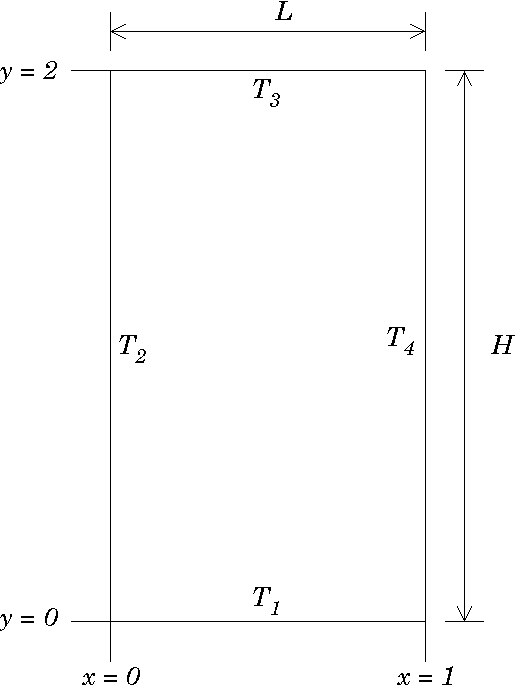
\includegraphics[width=3.5cm]{Hoffman.png}$$
			\end{column}
			\begin{column}{0.7\textwidth}
				\begin{eqnarray*}
					\nabla^2 T(\vec{x}) & = & 0 \,\,\,\,\, \text{para} \,\,\,\,\, \vec{x} \in [0,1] \times [0,2] \\
					T_1 & = & 100; T_2 = T_3 = T_4 = 0 
				\end{eqnarray*}
				Soluci\'on exacta: 
				
				$\displaystyle 
				T(\vec{x}) = T_1 \left[ 
				2\sum_{n=1}^{\infty} \frac{1-(-1)^n}{n \pi} 
				\frac{\sinh \left( \frac{n \pi (H-y)}{L} \right)}
				{\sinh \left( \frac{n \pi H}{L} \right)} 
				\sin \left( \frac{n \pi x}{L} \right)
				\right]
				$
			\end{column}
		\end{columns}

(\texttt{Poisson2D\_01.py, INPUT\_03})
}


%{\footnotesize{
%\begin{itemize}
%\item Dominio
%\begin{columns}
%\begin{column}{0.3\textwidth}
%$$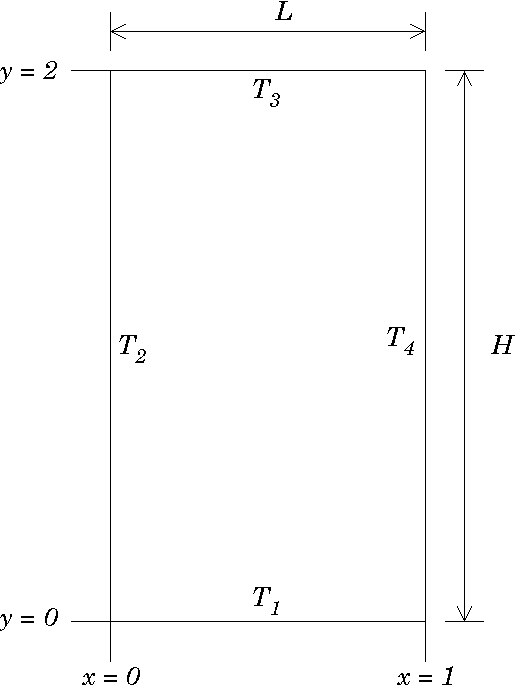
\includegraphics[width=2.5cm]{Hoffman.png}$$
%\end{column}
%\begin{column}{0.3\textwidth}
%$$\includegraphics[width=2.5cm]{HoffmanExact.png}$$
%\end{column}
%\begin{column}{0.3\textwidth}
%$$\includegraphics[width=3cm]{HoffmanExactS.png}$$
%\end{column}
%\end{columns}
%\item Ecuaci\'on y condiciones de frontera
%\begin{eqnarray*}
%\nabla^2 T(\Vector{x}) & = & 0 \,\,\,\,\, \text{para} \,\,\,\,\, \Vector{x} \in [0,1] \times [0,2] \\
%T_1 & = & 100; T_2 = T_3 = T_4 = 0 \,\,\,\,\, \text{(Cond. de frontera)} 
%\end{eqnarray*}
%\item Soluci\'on exacta: 
%$\displaystyle
%  T(\Vector{x}) = T_1 \left[ 
%    2\sum_{n=1}^{\infty} \frac{1-(-1)^n}{n \pi} 
%    \frac{\sinh \left( \frac{n \pi (H-y)}{L} \right)}
%    {\sinh \left( \frac{n \pi H}{L} \right)} 
%    \sin \left( \frac{n \pi x}{L} \right)
%    \right]
%$
%
%\end{itemize}
%}}

\end{frame}


\subsection{Problemas no estacionarios}

\begin{frame}{Problema no estacionario : Difusi\'on}

Encontrar $u(x,t)$ que cumpla:
\[
\frac{\partial u}{\partial t} = \frac{\partial}{\partial x} \left( \kappa \frac{\partial u}{\partial x} \right),
\,\,\, \text{ para } \,\,\, a \leq x \leq b, \,\,\, \text{ y } \,\,\, 0 \leq t \leq T_{max}.
\]

Condiciones iniciales: $u(x,0) = \alpha(x)$

Condiciones de frontera: $u(a,t)=A(t)$ y $u(b,t)=B(t)$

\pause

\begin{itemize}[<+->]
\item Cuando $\kappa = constante$, se tiene

\[
\frac{\partial u}{\partial t} = \kappa \frac{\partial^2 u}{\partial x^2},
\,\,\, \text{ para } \,\,\, a \leq x \leq b, \,\,\, \text{ y } \,\,\, 0 \leq t \leq T_{max}.
\]

\item Si $N_x$ es el n\'umero de inc\'ognitas en $x$, y $N_t$ es el n\'umero de pasos en el tiempo, entonces se definen
$\displaystyle \Delta x = \frac{b-a}{N_x + 1} = h$ y $\displaystyle \Delta t = \frac{T_{max}}{N_t} = h_t$, como el tama\~no de la malla y el paso de tiempo, respectivamente.
\end{itemize}

\end{frame}

\begin{frame}{Problema no estacionario: semidiscretizaci\'on}

\begin{columns}
\begin{column}{0.65\textwidth}
{\small Dado que
$\left.\dfrac{\partial^2 u}{\partial x^2}\right|_i =
(u_{xx})_i = (u_{i+1} - 2 u_{i} + u_{i-1})/\Delta x^2$ 
}
\end{column}
\begin{column}{0.35\textwidth}
$$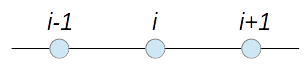
\includegraphics[width = 4cm]{Stencil1D_DF_01}$$
\end{column}
\end{columns}

\pause

Entonces tenemos que resolver el Problema de Valor Inicial:

\[
\boxed{\left.\frac{\partial u}{\partial t}\right|_i = f(t, u_{i+1}, u_{i}, u_{i-1}), \,\,\, 0 \leq t \leq T_{max}, \,\,\, \text{ con } u(x_i, 0) = \alpha(x_i)}
\]

donde $f(t, u_{i+1}, u_{i}, u_{i-1}) = \kappa (u_{i+1} - 2 u_{i} + u_{i-1}) / \Delta x^2$, para cada $i$ de la malla espacial (y en su caso condiciones frontera).

\end{frame}

\begin{frame}{Problema no estacionario: Euler hacia adelante (expl\'icito)}

El problema
\[
\left.\frac{\partial u}{\partial t}\right|_i = f(t, u_{i+1}, u_{i}, u_{i-1})
\]
para $0 \leq t \leq T_{max}$, con condici\'on inicial $u(x_i, 0) = \alpha(x_i) \equiv \alpha_i$ \pause se puede resolver usando el m\'etodo de Euler hacia adelante:

\[
\left.\frac{\partial u}{\partial t}\right|_i  \approx \frac{u_{i}^{n+1} - u_{i}^{n}}{\Delta t}
\]

donde $u_{i}^{n} \equiv u(x_i, t_n)$ y $u_{i}^{n+1} \equiv u(x_i, t_n + \Delta t)$. \pause Finalmente:

\[
u_{i}^{n+1} = u_{i}^{n} + \Delta t \, f(t, u_{i+1}^{n}, u_{i}^{n}, u_{i-1}^{n}) 
\]

con $f(t, u_{i+1}^{n}, u_{i}^{n}, u_{i-1}^{n}) = \dfrac{\Delta t}{\Delta x^2} \kappa (u_{i+1}^{n} - 2 u_{i}^{n} + u_{i-1}^{n}) $

\end{frame}

\begin{frame}{Problema no estacionario: Euler hacia adelante (expl\'icito)}
	
	$$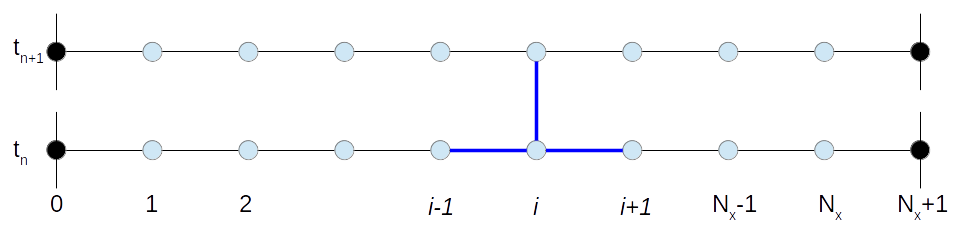
\includegraphics[width=10cm]{Stencil1D_DF_02.png}$$
	
	\begin{small}
		
		F\'ormula general:
		\begin{displaymath}
		u_{i}^{n+1} = u_{i}^{n} + \frac{h_t}{h^2} \kappa \left(u_{i+1}^{n} - 2 u_{i}^{n} + u_{i-1}^{n}\right)
		\end{displaymath}	
		
		
		Condiciones de frontera Dirichlet $u_{0}^{n} = A^{n}$ y $u_{N_x+1}^{n} = B^{n}$
	\end{small}
		\begin{enumerate}[<+->]
			\item {\footnotesize $u_{1}^{n+1} = u_{1}^{n} + \dfrac{h_t}{h^2} \kappa \left(u_{2}^{n} - 2 u_{1}^{n} + u_{0}^{n}\right) = u_{1}^{n} + \dfrac{h_t}{h^2} \kappa \left(u_{2}^{n} - 2 u_{1}^{n} + \boxed{A^{n}}\right)$}
			\item {\footnotesize $u_{N_x}^{n+1} = u_{N_x}^{n} + \dfrac{h_t}{h^2} \kappa \left(u_{N_x+1}^{n} - 2 u_{N_x}^{n} + u_{N_x-1}^{n}\right) = u_{N_x}^{n} + \dfrac{h_t}{h^2} \kappa \left(\boxed{B^{n}} - 2 u_{N_x}^{n} +  u_{N_x-1}^{n} \right)$}
		\end{enumerate}
		

\end{frame}

\begin{frame}{Problema no estacionario: Euler hacia adelante (expl\'icito)}


\begin{footnotesize}

\begin{block}{Algoritmo: Forward Euler (Cond. Dirichlet)}
INPUT: $a,b$, $N_x$, $h_t$, $N_t$ (o $T_{max}$), $\alpha_i$ para $i=1,\dots N_x$.

OUTPUT: $w_i^n$ para $i=0,\dots N_x+1$ y $ n = 0, \dots, N_t-1$

$w_{i}^{0} \leftarrow \alpha_{i}$ para $i=1,\dots N_x$

$w_0^{0} \leftarrow A$

$w_{N_x+1}^0 \leftarrow B$

DEF $f(t, w_{i+1}^{n}, w_{i}^{n}, w_{i-1}^{n}) : $
  RETURN $\left(u_{i+1}^{n} - 2 u_{i}^{n} + u_{i-1}^{n}\right) / h^2$

FOR $ n = 0$ TO $N_t-1$ DO
\begin{eqnarray*}
w_{i}^{n+1} & = & w_{i}^{n} + h_t \, f(t, w_{i+1}^{n}, w_{i}^{n}, w_{i-1}^{n}) \text{ para } 
i=1,\dots N_x \\
\text{plot} & \leftarrow & w_i^{n+1} \\
w_{i}^{n} & \leftarrow & w_{i}^{n+1}
\end{eqnarray*}
\end{block}
\end{footnotesize}

\end{frame}

\begin{frame}{Problema no estacionario: Euler hacia adelante (expl\'icito)}
	
	$$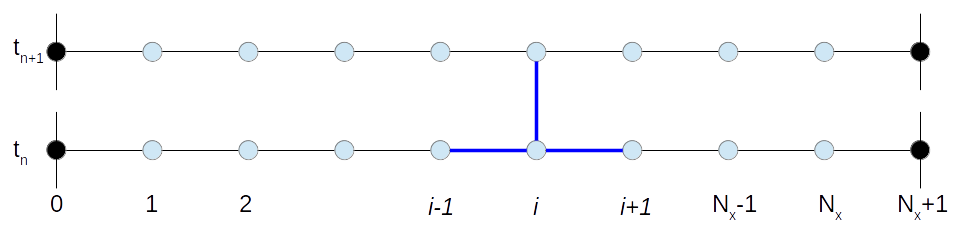
\includegraphics[width=10cm]{Stencil1D_DF_02.png}$$
	
	\begin{small}
		
		F\'ormula general:
		\begin{displaymath}
		u_{i}^{n+1} = u_{i}^{n} + \frac{h_t}{h^2} \kappa \left(u_{i+1}^{n} - 2 u_{i}^{n} + u_{i-1}^{n}\right)
		\end{displaymath}	
		
		
		Condiciones de frontera Dirichlet + Neumman $u_{0}^{n} = A^{n}$ y
		 $\displaystyle \left.\frac{\partial u}{\partial n}\right|_{N_x+1}^{n} = B^{n}$:
		 
		Aproximaci\'on ($\mathcal{O}(\Delta x)$): $u_{N_x+1}^{n} = h_t * B^n + u_{N_x}^{n}$
	\end{small}
			
		{\footnotesize $ \Rightarrow u_{N_x}^{n+1} = u_{N_x}^{n} + \dfrac{h_t}{h^2} \kappa \left(\boxed{u_{N_x+1}^{n}} - 2 u_{N_x}^{n} + u_{N_x-1}^{n}\right) = u_{N_x}^{n} + \dfrac{h_t}{h^2} \kappa \left(h_t * B^{n} - u_{N_x}^{n} +  u_{N_x-1}^{n} \right)$}

		

\end{frame}

\begin{frame}{Problema no estacionario: Euler hacia adelante (expl\'icito)}
	
	\begin{footnotesize}
		
		\begin{block}{Algoritmo: Forward Euler (Cond. Dirichlet + Neumman)}
			INPUT: $a,b$, $N_x$, $h_t$, $N_t$ (o $T_{max}$), $\alpha_i$ para $i=1,\dots N_x$.
			
			OUTPUT: $w_i^n$ para $i=0,\dots N_x+1$ y $ n = 0, \dots, N_t-1$
			
			$w_{i}^{0} \leftarrow \alpha_{i}$ para $i=1,\dots N_x$
			
			$w_0^{0} \leftarrow A$

DEF $f(t, w_{i+1}^{n}, w_{i}^{n}, w_{i-1}^{n}) : $
RETURN $\left(u_{i+1}^{n} - 2 u_{i}^{n} + u_{i-1}^{n}\right) / h^2$
			
			FOR $ n = 0$ TO $N_t-1$ DO
			\begin{eqnarray*}
				w_{N_x+1}^n & = & h_t * B^n + w_{N_x}^n \\
				w_{i}^{n+1} & = & w_{i}^{n} + h_t \, f(t, w_{i+1}^{n}, w_{i}^{n}, w_{i-1}^{n}) \text{ para } 
				i=1,\dots N_x \\
				\text{plot} & \leftarrow & w_i^{n+1} \\
				w_{i}^{n} & \leftarrow & w_{i}^{n+1}
			\end{eqnarray*}
		\end{block}
	\end{footnotesize}
	
\end{frame}


\begin{frame}{Problema no estacionario: Euler hacia atr\'as (impl\'icito)}

El problema
\[
\left.\frac{\partial u}{\partial t}\right|_i = f(t, u_{i+1}, u_{i}, u_{i-1})
\]
para $0 \leq t \leq T_{max}$, con condici\'on inicial $u(x_i, 0) = \alpha(x_i) \equiv \alpha_i$ \pause se puede resolver usando el m\'etodo de Euler hacia atr\'as:

\[
\left.\frac{\partial u}{\partial t}\right|_i  \approx \frac{u_{i}^{n} - u_{i}^{n-1}}{\Delta t}
\]

donde $u_{i}^{n} \equiv u(x_i, t_n)$ y $u_{i}^{n-1} \equiv u(x_i, t_n - \Delta t)$. \pause Finalmente:

\[
u_{i}^{n} = u_{i}^{n-1} + \Delta t \, f(t, u_{i+1}^{n}, u_{i}^{n}, u_{i-1}^{n}) 
\]

\pause

F\'ormula impl\'icita para encontrar $u_i^{n}$, para $1 \leq n \leq N_t$:
\[
\boxed{u_{i}^{n} = u_{i}^{n-1} + \frac{\Delta t}{\Delta x^2} \kappa (u_{i+1}^{n} - 2 u_{i}^{n} + u_{i-1}^{n})}
\]
\end{frame}


\begin{frame}{Problema no estacionario: Euler hacia atr\'as (impl\'icito)}
	
	$$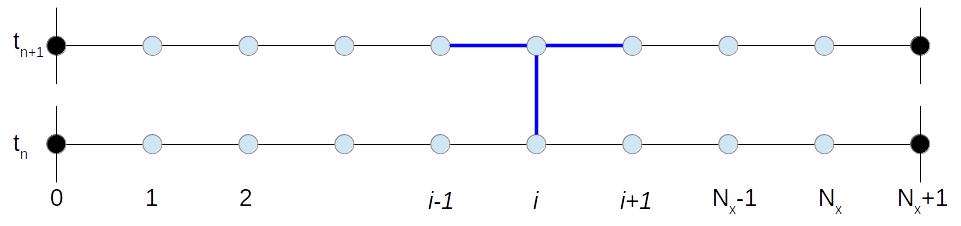
\includegraphics[width=10cm]{Stencil1D_DF_03.png}$$
	
	\begin{small}
		
		F\'ormula general:
		\begin{displaymath}
		u_{i}^{n+1} = u_{i}^{n} + \frac{h_t}{h^2} \kappa \left(u_{i+1}^{n+1} - 2 u_{i}^{n+1} + u_{i-1}^{n+1}\right)
		\end{displaymath}	
		
		
		La f\'ormula es impl\'icita, se debe resolver un sistema de ecuaciones, pero es m\'as estable que el m\'etodo hacia adelante.
	\end{small}
	
\end{frame}

\begin{frame}{Problema no estacionario: Euler hacia atr\'as (impl\'icito)}

Sistema de ecuaciones
\begin{eqnarray*}
u_{1}^{n} & = & u_{1}^{n-1} + \frac{\Delta t}{\Delta x^2} \kappa \left(u_{2}^{n} - 2 u_{1}^{n} + \boxed{u_{0}^{n}}\right) \,\,\, \mbox{ Cond. de frontera}\\
u_{2}^{n} & = & u_{2}^{n-1} + \frac{\Delta t}{\Delta x^2} \kappa \left(u_{3}^{n} - 2 u_{2}^{n} + u_{1}^{n}\right) \\
\dots & \dots & \dots \\
u_{i}^{n} & = & u_{i}^{n-1} + \frac{\Delta t}{\Delta x^2} \kappa \left(u_{i+1}^{n} - 2 u_{i}^{n} + u_{i-1}^{n}\right) \\
\dots & \dots & \dots \\
u_{N}^{n} & = & u_{N}^{n-1} + \frac{\Delta t}{\Delta x^2} \kappa \left(\boxed{u_{N+1}^{n}} - 2 u_{N}^{n} + u_{N-1}^{n}\right) \,\,\, \mbox{ Cond. de frontera}\\
\end{eqnarray*}
\pause
Condiciones de frontera:
\begin{eqnarray*}
u_{1}^{n} & = & u_{1}^{n-1} + \frac{\Delta t}{\Delta x^2} \kappa \left(u_{2}^{n} - 2 u_{1}^{n} + \boxed{A^{n}}\right) \,\,\,\,\, \mbox{(Dirichlet)} \\
u_{N}^{n} & = & u_{N}^{n-1} + \frac{\Delta t}{\Delta x^2} \kappa \left(\boxed{\Delta x B^{n} + u_{N}^{n}} - 2 u_{N}^{n} + u_{N-1}^{n}\right) \,\,\,\,\, \mbox{(Neumman)}\\
\end{eqnarray*}

\end{frame}

\begin{frame}{Problema no estacionario: Euler hacia atr\'as (impl\'icito)}

\begin{footnotesize}
Definimos: $\displaystyle r \equiv \frac{\Delta t}{\Delta x^2} \kappa$ entonces escribimos el sistema de ecuaciones anterior como sigue:

\begin{eqnarray*}
-r u_{2}^{n} + (1+2r) u_{1}^{n} & = & u_{1}^{n-1} + r A^{n}\\
-r u_{3}^{n} + (1+2r) u_{2}^{n} - r u_{1}^{n} & = & u_{2}^{n-1} \\
\dots & \dots & \dots \\
-r u_{i+1}^{n} + (1+2r) u_{i}^{n} - r u_{i-1}^{n} & = & u_{i}^{n-1} \\
\dots & \dots & \dots \\
(1+r) u_{N}^{n} - r u_{N-1}^{n} & = & u_{N}^{n-1} + r \Delta x B^{n}\\
\end{eqnarray*}
\pause 
En forma matricial:
\[
\left[
\begin{matrix}
(1+2r) & -r     & 0      & 0      & 0      & 0  \\
-r     & (1+2r) & -r     & 0      & 0      & 0  \\
0      & -r     & (1+2r) & -r     & 0      & 0  \\
0      & 0      & -r     & (1+2r) & -r     & 0  \\
\vdots & \vdots & \vdots & \vdots & \ddots & \vdots \\
0      & 0      & 0      & 0      & -r     & (1+r) 
\end{matrix}
\right] \left[
\begin{matrix}
u_{1}^{n} \\ u_{2}^{n} \\u_{3}^{n} \\u_{4}^{n} \\ \vdots \\u_{N}^{n}
\end{matrix}
\right] = \left[
\begin{matrix}
u_{1}^{n-1} + rA^{n} \\ u_{2}^{n-1} \\u_{3}^{n-1} \\u_{4}^{n-1} \\ \vdots \\u_{N}^{n-1} + r\Delta x B^{n}
\end{matrix}
\right]
\]
\end{footnotesize}

\end{frame}

\begin{frame}{Estabilidad: Euler Forward vs. Euler Backward}

\begin{small}

\begin{columns}
\begin{column}{0.45\textwidth}
\textbf{Euler Forward (Expl\'icito)}

\begin{itemize}[<+->]
\item La evaluaci\'on de $u_i^{n+1}$ se realiza mediante la evaluaci\'on de una f\'ormula expl\'icita.
\item Cada una de estas evaluaciones es independiente de las otras, por lo que este esquema es paralelizable directamente.
\item Es condicionalmente estable: $\frac{\Delta t}{\Delta x^2} \kappa < \frac{1}{2} \Longrightarrow \Delta t < \frac{\Delta x^2}{2 \kappa}$.
\item La condici\'on anterior obliga a realizar muchos pasos de tiempo para llegar a $T_{max}$.
\end{itemize}
\end{column}
\begin{column}{0.45\textwidth}
\textbf{Euler Backward (Impl\'icito)}
\begin{itemize}[<+->]
\item La soluci\'on en el paso $n+1$ se encuentra resolviendo un sistema lineal de ecuaciones.
\item Es posible paralelizar la soluci\'on del sistema lineal.
\item Es incondicionalmente estable, por lo que $\Delta t$ puede ser grande.
\item Si la matriz del sistema est\'a mal condicionada, la soluci\'on de un paso de tiempo puede tardar mucho.
\end{itemize}
\end{column}
\end{columns}

\begin{itemize}[<+->]
\item En ambos casos el orden de la aproximaci\'on es $\mathcal{O}(\Delta x^2) + \mathcal{O}(\Delta t)$.
\end{itemize}
\end{small}

\end{frame}

\begin{frame}{Convergencia, consistencia y estabilidad}
\begin{itemize}[<+->]
\item \textbf{Convergencia} : 
Es la propiedad de un m\'etodo num\'erico de producir una soluci\'on 
que aproxima a la soluci\'on exacta conforme la distancia entre los 
puntos de la malla tiende a cero. 
\item \textbf{Consistencia} :
Un esquema num\'erico consistente produce sistemas de ecuaciones 
algebraicas equivalentes a las ecuaciones gobernantes originales 
cuando el espaciamiento de los nodos de la malla tiende a cero. 
\item \textbf{Estabilidad}
La estabilidad est\'a asociada con la amortiguaci\'on del error 
conforme el m\'etodo num\'erico procede. 
\end{itemize}

\pause

\begin{block}{Teorema de equivalencia de Lax}
Para problemas lineales una condici\'on necesaria y suficiente 
para obtener convergencia es que el m\'etodo sea consistente y estable. 
\end{block}

\end{frame}

\begin{frame}{Problema no estacionario: Crank-Nicholson (impl\'icito)}

$$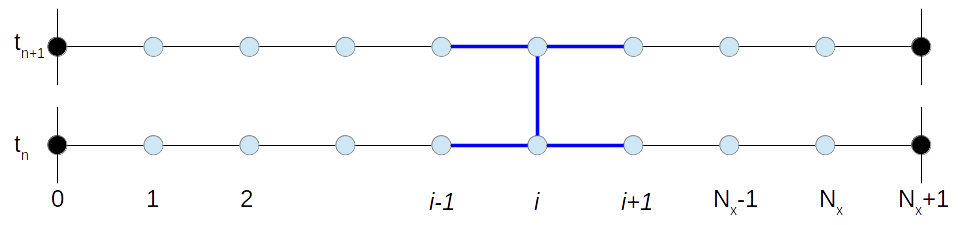
\includegraphics[width=10cm]{Stencil1D_DF_04.png}$$

\begin{small}
	
Esquema con la propiedad  en $\mathcal{O}(\Delta x^2 + \Delta t^2)$. Aproximamos en $(x_i,t^{n+\frac{1}{2}})$:
	\begin{eqnarray*}
	\left.\dfrac{\partial u}{\partial t}\right|_{i}^{n+\frac{1}{2}} & = & \dfrac{u_{i}^{n+1} - u_{n}}{h_t} \\ 	
	 \left.\dfrac{\partial^2 u}{\partial x^2}\right|_{i}^{n+\frac{1}{2}} & = & \frac{1}{2 h^2}  \left(u_{i+1}^{n+1} - 2 u_{i}^{n+1} + 
	u_{i-1}^{n+1} + u_{i+1}^{n} - 2 u_{i}^{n} + u_{i-1}^{n}\right)
	\end{eqnarray*}	
	\begin{displaymath}
	\boxed{u_{i}^{n+1} -  \frac{h_t}{2 h^2}  \kappa \left(u_{i+1}^{n+1} - 2 u_{i}^{n+1} + 
	u_{i-1}^{n+1}\right) = u_{i}^{n} + \frac{h_t}{2 h^2}  \kappa \left(u_{i+1}^{n} - 2 u_{i}^{n} + u_{i-1}^{n}\right)}
	\end{displaymath}
	La f\'ormula es impl\'icita y es estable.
	
\end{small}

\end{frame}


\begin{frame}{Ejemplo : Ecuaci\'on de calor en 2D}

\begin{columns}
	\begin{column}{0.3\textwidth}
		$$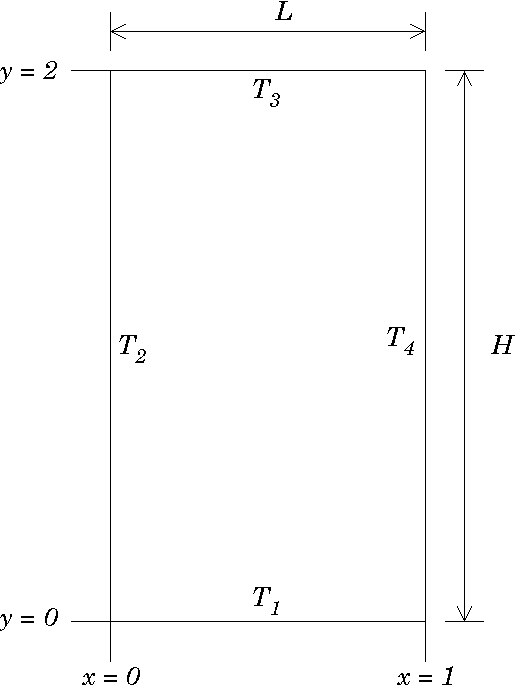
\includegraphics[width=2.5cm]{Hoffman.png}$$
	\end{column}
	\begin{column}{0.3\textwidth}
		$$\includegraphics[width=2.5cm]{HoffmanExact.png}$$
	\end{column}
	\begin{column}{0.3\textwidth}
		$$\includegraphics[width=3cm]{HoffmanExactS.png}$$
	\end{column}
\end{columns}

{\footnotesize{
\begin{itemize}
\item Ecuaci\'on y condiciones iniciales y de frontera
\begin{eqnarray*}
\frac{\partial T(\Vector{x},t)}{\partial t} & = & \nabla^2 T(\Vector{x}, t) \,\,\,\,\, \text{para} \,\,\,\,\, \Vector{x} \in [0,1] \times [0,2]  \,\,\, \text{y} \,\,\, 0 \leq t \leq T_{max} \\
T_1 & = & 100; T_2 = T_3 = T_4 = 0 \,\,\,\,\, \text{(Cond. de frontera)} \\
T(\Vector{x}, 0) & = & 0 \,\,\,\,\, \text{para} \,\,\,\,\, \Vector{x} \in (0,1) \times (0,2) \,\,\, \text{(Cond. inicial)} 
\end{eqnarray*}
\item Soluci\'on exacta: similar a la soluci\'on del caso estacionario cuando $t \rightarrow \infty$.

\end{itemize}
}}

\end{frame}


\begin{frame}{Problema no estacionario: Advecci\'on}

Encontrar $u(x,t)$ que cumpla:
\[
\frac{\partial u}{\partial t} +  c \frac{\partial u}{\partial x}  = 0,
\,\,\, \text{ para } \,\,\, a \leq x \leq b, \,\,\, \text{ y } \,\,\, 0 \leq t \leq T_{max}.
\]

\begin{itemize}[<+->]
	\item Cond. inicial: $u(x,0) = \eta(x)$ ( + conds. de frontera $\Longrightarrow$ sol. \'unica).
	\item Problema de Cauchy (PVI): 
	\begin{itemize}
		\item $-\infty \leq x \leq \infty$ 
		\item Solo requiere de la condici\'on inicial.
		\item El perfil inicial se mueve a velocidad $c$, es decir: $u(x,0) = \eta(x - c * t)$
	\end{itemize}

\end{itemize}

\end{frame}

\begin{frame}{Esquemas de aproximaci\'on para Advecci\'on ($\left|\frac{c h_t}{h}\right| \leq 1$)}

\begin{itemize}[<+->]
	\item Orden de aprox. $\mathcal{O}(\Delta x^2 + \Delta t)$: 
\begin{displaymath}
u_{i}^{n+1} = u_{i}^{n} - \dfrac{c h_t}{2 h}\left(u_{i+1}^{n} - u_{i-1}^{n} \right)
\end{displaymath}	
	\item \textit{Lax-Friedrichs Method} :
\begin{displaymath}
u_{i}^{n+1} =  \dfrac{1}{2}\left(u_{i-1}^{n} + u_{i+1}^{n}\right) - \dfrac{c h_t}{2 h}\left(u_{i+1}^{n} - u_{i-1}^{n} \right)
\end{displaymath}		
	\item \textit{Leapfrog Method} :
\begin{displaymath}
u_{i}^{n+1} =  u_{i}^{n-1} - \dfrac{c h_t}{2 h}\left(u_{i+1}^{n} - u_{i-1}^{n} \right)
\end{displaymath}		
	\item \textit{Lax-Wendroff Method} :
\begin{displaymath}
u_{i}^{n+1} = u_{i}^{n} - \dfrac{c h_t}{2 h}\left(u_{i+1}^{n} - u_{i-1}^{n} \right) + \dfrac{c^2 h_t^2}{2 h^2}\left(u_{i+1}^{n} - 2u_{i}^{n} + u_{i-1}^{n} \right)
\end{displaymath}	
 ({\footnotesize $u(x,t+\delta t) = u(x,t) + h_t u_t(x,t) + \frac{h_t^2}{2} u_{tt}(x,t)+\dots  $})

\end{itemize}

\end{frame}
	
\begin{frame}{Esquemas de aproximaci\'on para Advecci\'on }

\begin{itemize}[<+->]
	\item Upwind $c > 0$ (Estabilidad: $0 \leq \frac{c h_t}{h} \leq 1$): 
\begin{displaymath}
u_{i}^{n+1} = u_{i}^{n} - \dfrac{c h_t}{2 h}\left(u_{i}^{n} - u_{i-1}^{n} \right)
\end{displaymath}	
	\item Upwind $c < 0$ (Estabilidad: $-1 \leq \frac{c h_t}{h} \leq 0$): 
\begin{displaymath}
u_{i}^{n+1} = u_{i}^{n} - \dfrac{c h_t}{2 h}\left(u_{i+1}^{n} - u_{i}^{n} \right)
\end{displaymath}
	\item Beam-Warming $c > 0$ (Estabilidad: $0 \leq \frac{c h_t}{h} \leq 2$): 
\begin{displaymath}
u_{i}^{n+1} = u_{i}^{n} - \dfrac{c h_t}{2 h}\left(3u_{i}^{n} -4 u_{i-1}^{n} + u_{i-2}^n\right) + \dfrac{c^2 h_t^2}{2 h^2}\left(u_{i}^{n} - 2u_{i-1}^{n} + u_{i-2}^{n} \right)
\end{displaymath}	
	\item Beam-Warming $c < 0$ (Estabilidad: $-2 \leq \frac{c h_t}{h} \leq 0$): 
\begin{displaymath}
u_{i}^{n+1} = u_{i}^{n} - \dfrac{c h_t}{2 h}\left(-3u_{i}^{n} +4 u_{i+1}^{n} - u_{i+2}^n\right) + \dfrac{c^2 h_t^2}{2 h^2}\left(u_{i}^{n} - 2u_{i+1}^{n} + u_{i+2}^{n} \right)
\end{displaymath}	

\end{itemize}

\end{frame}


\begin{frame}{Difusi\'on num\'erica }

{\small En el m\'etodo de Lax-Friedichs podemos escribir:
\begin{displaymath}
 \dfrac{1}{2}\left(u_{i-1}^{n} + u_{i+1}^{n}\right) =  u_{i}^{n} + \dfrac{1}{2}\left(u_{i-1}^{n} - 2 u_{i}^{n} + u_{i+1}^{n}\right)
\end{displaymath}
Con lo que obtenemos:
\begin{displaymath}
u_{i}^{n+1} =  u_{i}^{n}  - \dfrac{c h_t}{2 h}\left(u_{i+1}^{n} - u_{i-1}^{n} \right) + \dfrac{1}{2}\left(u_{i-1}^{n} - 2 u_{i}^{n} + u_{i+1}^{n}\right)
\end{displaymath}		
Que se puede rearreglar como:
\begin{displaymath}
\left(\dfrac{u_{i}^{n+1} - u_{i}^{n}}{h_t}\right) + c\left(\dfrac{u_{i+1}^{n} - u_{i-1}^{n}}{2 h} \right) = \dfrac{h^2}{2h_t}\left(\dfrac{u_{i-1}^{n} - 2 u_{i}^{n} + u_{i+1}^{n}}{h^2}\right)
\end{displaymath}		
Esta \'ultima discretizaci\'on es similar a la obtenida de una ecuaci\'on como:
\begin{displaymath}
\dfrac{\partial u}{\partial t} + c \dfrac{\partial u}{\partial x} = \epsilon \dfrac{\partial^2 u}{\partial x^2}, \text{ para } \epsilon = h^2 / 2 h_t
\end{displaymath}
Para el m\'etodo de Upwind: $\epsilon = c h / 2$.

Para el m\'etodo de Lax-Wendroff: $\epsilon = c^2 h_t / 2$.
}

\end{frame}


\appendix
\section<presentation>*{\appendixname}
\subsection<presentation>*{Bibliograf\'{\i}a}

\begin{frame}[allowframebreaks]
  \frametitle<presentation>{Bibliograf\'{\i}a}
    
  \begin{thebibliography}{10}
   
% BOOKS 
  \beamertemplatebookbibitems

\bibitem{Herrera1} 
[1] I. Herrera and M. B. Allen and G. F. Pinder, 
\newblock {\em Numerical modeling in science and engineering}, 
\newblock John Wiley \& Sons., USA, 1988.
    
\bibitem{Herrera2} 
[2] I. Herrera and G. F. Pinder, 
\newblock {\em General principles of mathematical computational modeling}, 
\newblock {John Wiley}, in press.

\bibitem{Leveque}
[3] R.J. Leveque,
\newblock {\em Finite Difference Method for Ordinary and Partial Differential Equations: Steady State and Time-Dependent Problems },
\newblock {Society for Industrial and Applied Mathematics (SIAM), Philadelphia}, 2007.

\bibitem{Leveque}
[4] R.J. Leveque,
\newblock {\em Finite Volume Method for Hyperbolic Problems},
\newblock {Cambridge University Press}, 2004.

\bibitem{Saad}
[5] Y. Saad
    \newblock {\em Iterative Methods for Sparse Linear Systems}.
    \newblock PWS/ITP 1996.
    \newblock {Online: 
\textsf{http://www-users.cs.umn.edu/\textasciitilde saad/books.html}, 
      2000}

\bibitem{Burden}
[6]  Richard Burden and J. Douglas Faires
  \newblock{\em Numerical Analysis}
  \newblock International Thomson Publishing 1997
  
  \bibitem{Barret}
[7]    R. Barret, \textit{et al.}
    \newblock {\em Templates for the Solution of Linear Systems: 
      Building Blocks for Iterative Methods}
    \newblock {Online: \textsf{http://www.siam.org/books}.}

\bibitem{Patankar:1980}
[8]  S.~V. Patankar.
  \newblock {\em Numerical Heat Transfer and Fluid Flow}.
  \newblock {Mc\-Graw\---Hill}, 1980.

\bibitem{Versteeg:1995}
[9]  H.~Versteeg and W.~Malalasekera.
  \newblock {\em An introduction to computational fluid dynamics: The finite
    volume method}.
  \newblock Longman, 1995.

\bibitem{Chen2006}
[10]  Z.~Chen and G.~Huan and Y.~Ma,
  \newblock {\em Computational Methods for Multiphase Flows in Poros Media}, 
  Cap\'{\i}tulo 4.
  \newblock SIAM, 2006.
  
\bibitem{Fletcher2:1991}
[11]  C.~Fletcher.
  \newblock {\em Computational Techniques for Fluid Dynamics 1: Specific
    Techniques for Different Flow Categories}.
  \newblock Springer--Verlag, second edition edition, 1991.
  
\bibitem{Hirsch1:1988}
[12]  C.~Hirsch.
  \newblock {\em Numerical Computation of Internal and External Flows Volume 1:
    Fundamentals of Numerical Discretization}.
  \newblock John Wiley \& Sons, 1988.
  
\bibitem{Hirsch2:1988}
[13]  C.~Hirsch.
  \newblock {\em Numerical Computation of Internal and External Flows Volume 2:
    Computational Methods for Inviscid and Viscous Flows}.
  \newblock John Wiley \& Sons, 1988.
   

 \bibitem{Scarborough:1958}
[14]   J.~B. Scarborough.
   \newblock {\em Numerical Mathematical Analysis}.
   \newblock {4th ed., Johns Hopkins University Press}, 1958.

 % ARTICULOS    
    \beamertemplatearticlebibitems
    
  \bibitem{Han:1981}
[15]    T.~Han, J.~Humphrey, and B.~E. Launder.
    \newblock A comparison of hybrid and quadratic-upstream differencing in high
    reynolds number elliptic flows.
    \newblock {\em Comp. Meth. in App. Mech. and Eng.}, 29:81--95, 1981.
    
 \bibitem{Hayase:1992}
[16]   T.~Hayase, J.~Humphrey, and R.~Greif.
   \newblock A consistently formulated quick scheme for fast and stable
   convergence using finite-volume iterative calculation procedures.
   \newblock {\em J. of Comp. Phys}, 98:108--118, 1992.

 \bibitem{Huang:1985}
[17]   P.~G. Huang, B.~E. Launder, and M.~A. Leschziner.
   \newblock Discretization of non-linear convection processes: A broad-range
   comparison of four schemes.
   \newblock {\em Comp. Meth. in App. Mech. and Eng.}, 48:1--24, 1985.

 \bibitem{Leonard:1979}
[18]   B.~P. Leonard.
   \newblock A stable and accurate conevctive modelling procedure based on
   quadratic upstream interpolation.
   \newblock {\em Comp. Meth. in App. Mech. and Engineering}, 19:59--98, 1979.
  
 \bibitem{Pollar:1982}
[19]   A.~Pollard and A.~L. Siu.
   \newblock The calcualtion of some laminar flows using various discretization
   schemes.
   \newblock {\em Comp. Meth. in App. Mech. and Eng.}, 35:293--313, 1982.
   
  \end{thebibliography}
\end{frame}

\end{document}

